\documentclass{beamer}

\usepackage[utf8]{inputenc}
\usepackage[portuguese]{babel}
\usepackage{graphicx}

\usetheme{Warsaw}

\title{Article Presentation}
\subtitle{A Robot Application for Marine Vessel Inspection}

\author{Mateus Santos de Cerqueira}
\institute{SENAI}
\date{\today}

\begin{document}
    \begin{frame}
        \titlepage
    \end{frame}
    
    \section{A Robot Application for Marine Vessel Inspection}

        \subsection{INTRODUCTION}

            \begin{frame}{INTRODUCTION}
                \begin{figure}[htb]
                    \centering
                    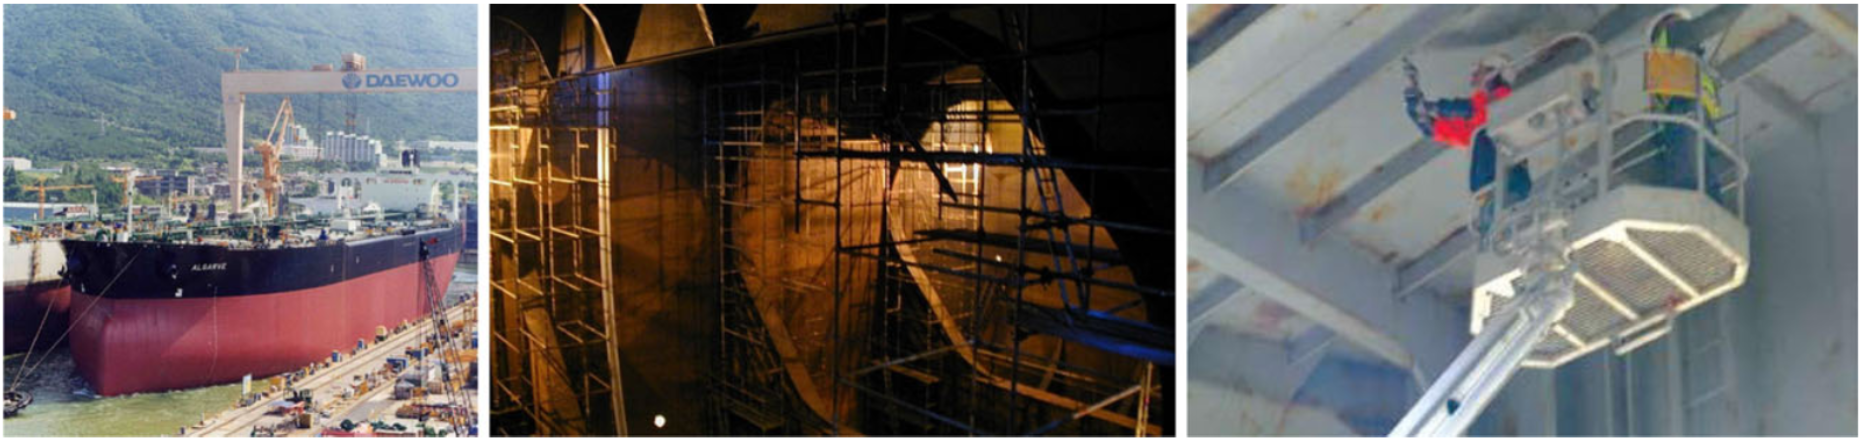
\includegraphics[scale=0.16]{figuras/traditional_inspection.png}                   
                    \label{}
                \end{figure}
                Overview \\
                Traditional Inspection \\
                MINOAS \\
                Spatial Content Management System (SCMS)                           
            \end{frame}
            
        \subsection{REENGINEERED INSPECTION PROCEDURE}

            \begin{frame}{REENGINEERED INSPECTION PROCEDURE}
                \begin{figure}[htb]
                    \centering
                    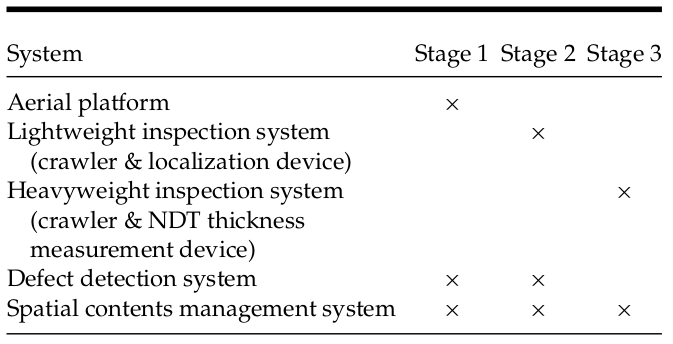
\includegraphics[scale=0.35]{figuras/inspection_stages}                   
                    \label{}
                \end{figure}
                Fast visual inspection \\
                Visual close-up survey \\
                Thickness measurement collection
            \end{frame}

        \subsection{MINOAS INSPECTION PLATFORMS}

            \begin{frame}{MINOAS Inspecton Platforms}
                o terceiro frame            
            \end{frame}

        \subsection{A VISION-BASED SOLUTION FOR DEFECT DETECTION}

            \begin{frame}{A VISION-BASED SOLUTION FOR DEFECT DETECTION}
                o quarto frame            
            \end{frame}            

        \subsection{SPATIAL CONTENT MANAGEMENT SYSTEM FOR ROBOT-ACQUIRED INSPECTION DATA}

            \begin{frame}{SPATIAL CONTENT MANAGEMENT SYSTEM FOR ROBOT-ACQUIRED INSPECTION DATA}
                o quinto frame            
            \end{frame}        

        \subsection{SYSTEM PERFORMANCE EVALUATION}

            \begin{frame}{SYSTEM PERFORMANCE EVALUATION}
                o sexto frame            
            \end{frame}
            
        \subsection{CONCLUSION AND FUTURE RESEARCH}

            \begin{frame}{CONCLUSION AND FUTURE RESEARCH}
                o setimo frame            
            \end{frame}

\end{document}
